% !Mode:: "TeX:UTF-8"
\documentclass[QAofGroup.tex]{subfiles}

\begin{document}
%-=-=-=-=-=-=-=-=-=-=-=-=-=-=-=-=-=-=-=-=-=-=-=-=
%
%	CHAPTER
%
%-=-=-=-=-=-=-=-=-=-=-=-=-=-=-=-=-=-=-=-=-=-=-=-=

%%================================================================
\chapter{20180109}\label{ch180109}
%----------------------------------------------------------------------------------------

\begin{qst}\label{Q2018010901}
请问tikz如何标注角度呢?\index{标注角度}
\end{qst}
\ans \verb|\draw [-stealth] (0.5,0) arc(0:135:0.5cm)  node[right]{$\alpha$} ;|

\includegraphics[width=0.5\textwidth]{pic14.png}

\begin{qst}\label{Q2018010902}
\verb|\mathcal{\bm M}|就是黑不了,咋整?
\end{qst}
\ans \verb|\bm{\mathcal{M}}| 这样试一下。!

可以调用宏包

\verb|\usepackage{bm,dsfont} %\bm, \mathds|

\verb|\usepackage[mathscr]{eucal}% \mathscr and \mathcal|

\begin{qst}\label{Q2018010903}
话说怎么调用本地文件夹的字体,不打算直接装到系统里面,懒得再刷新字体缓存了。\index{调用本地字体}
\end{qst}
\ans
以前看到过相关的例子,可以参考下。


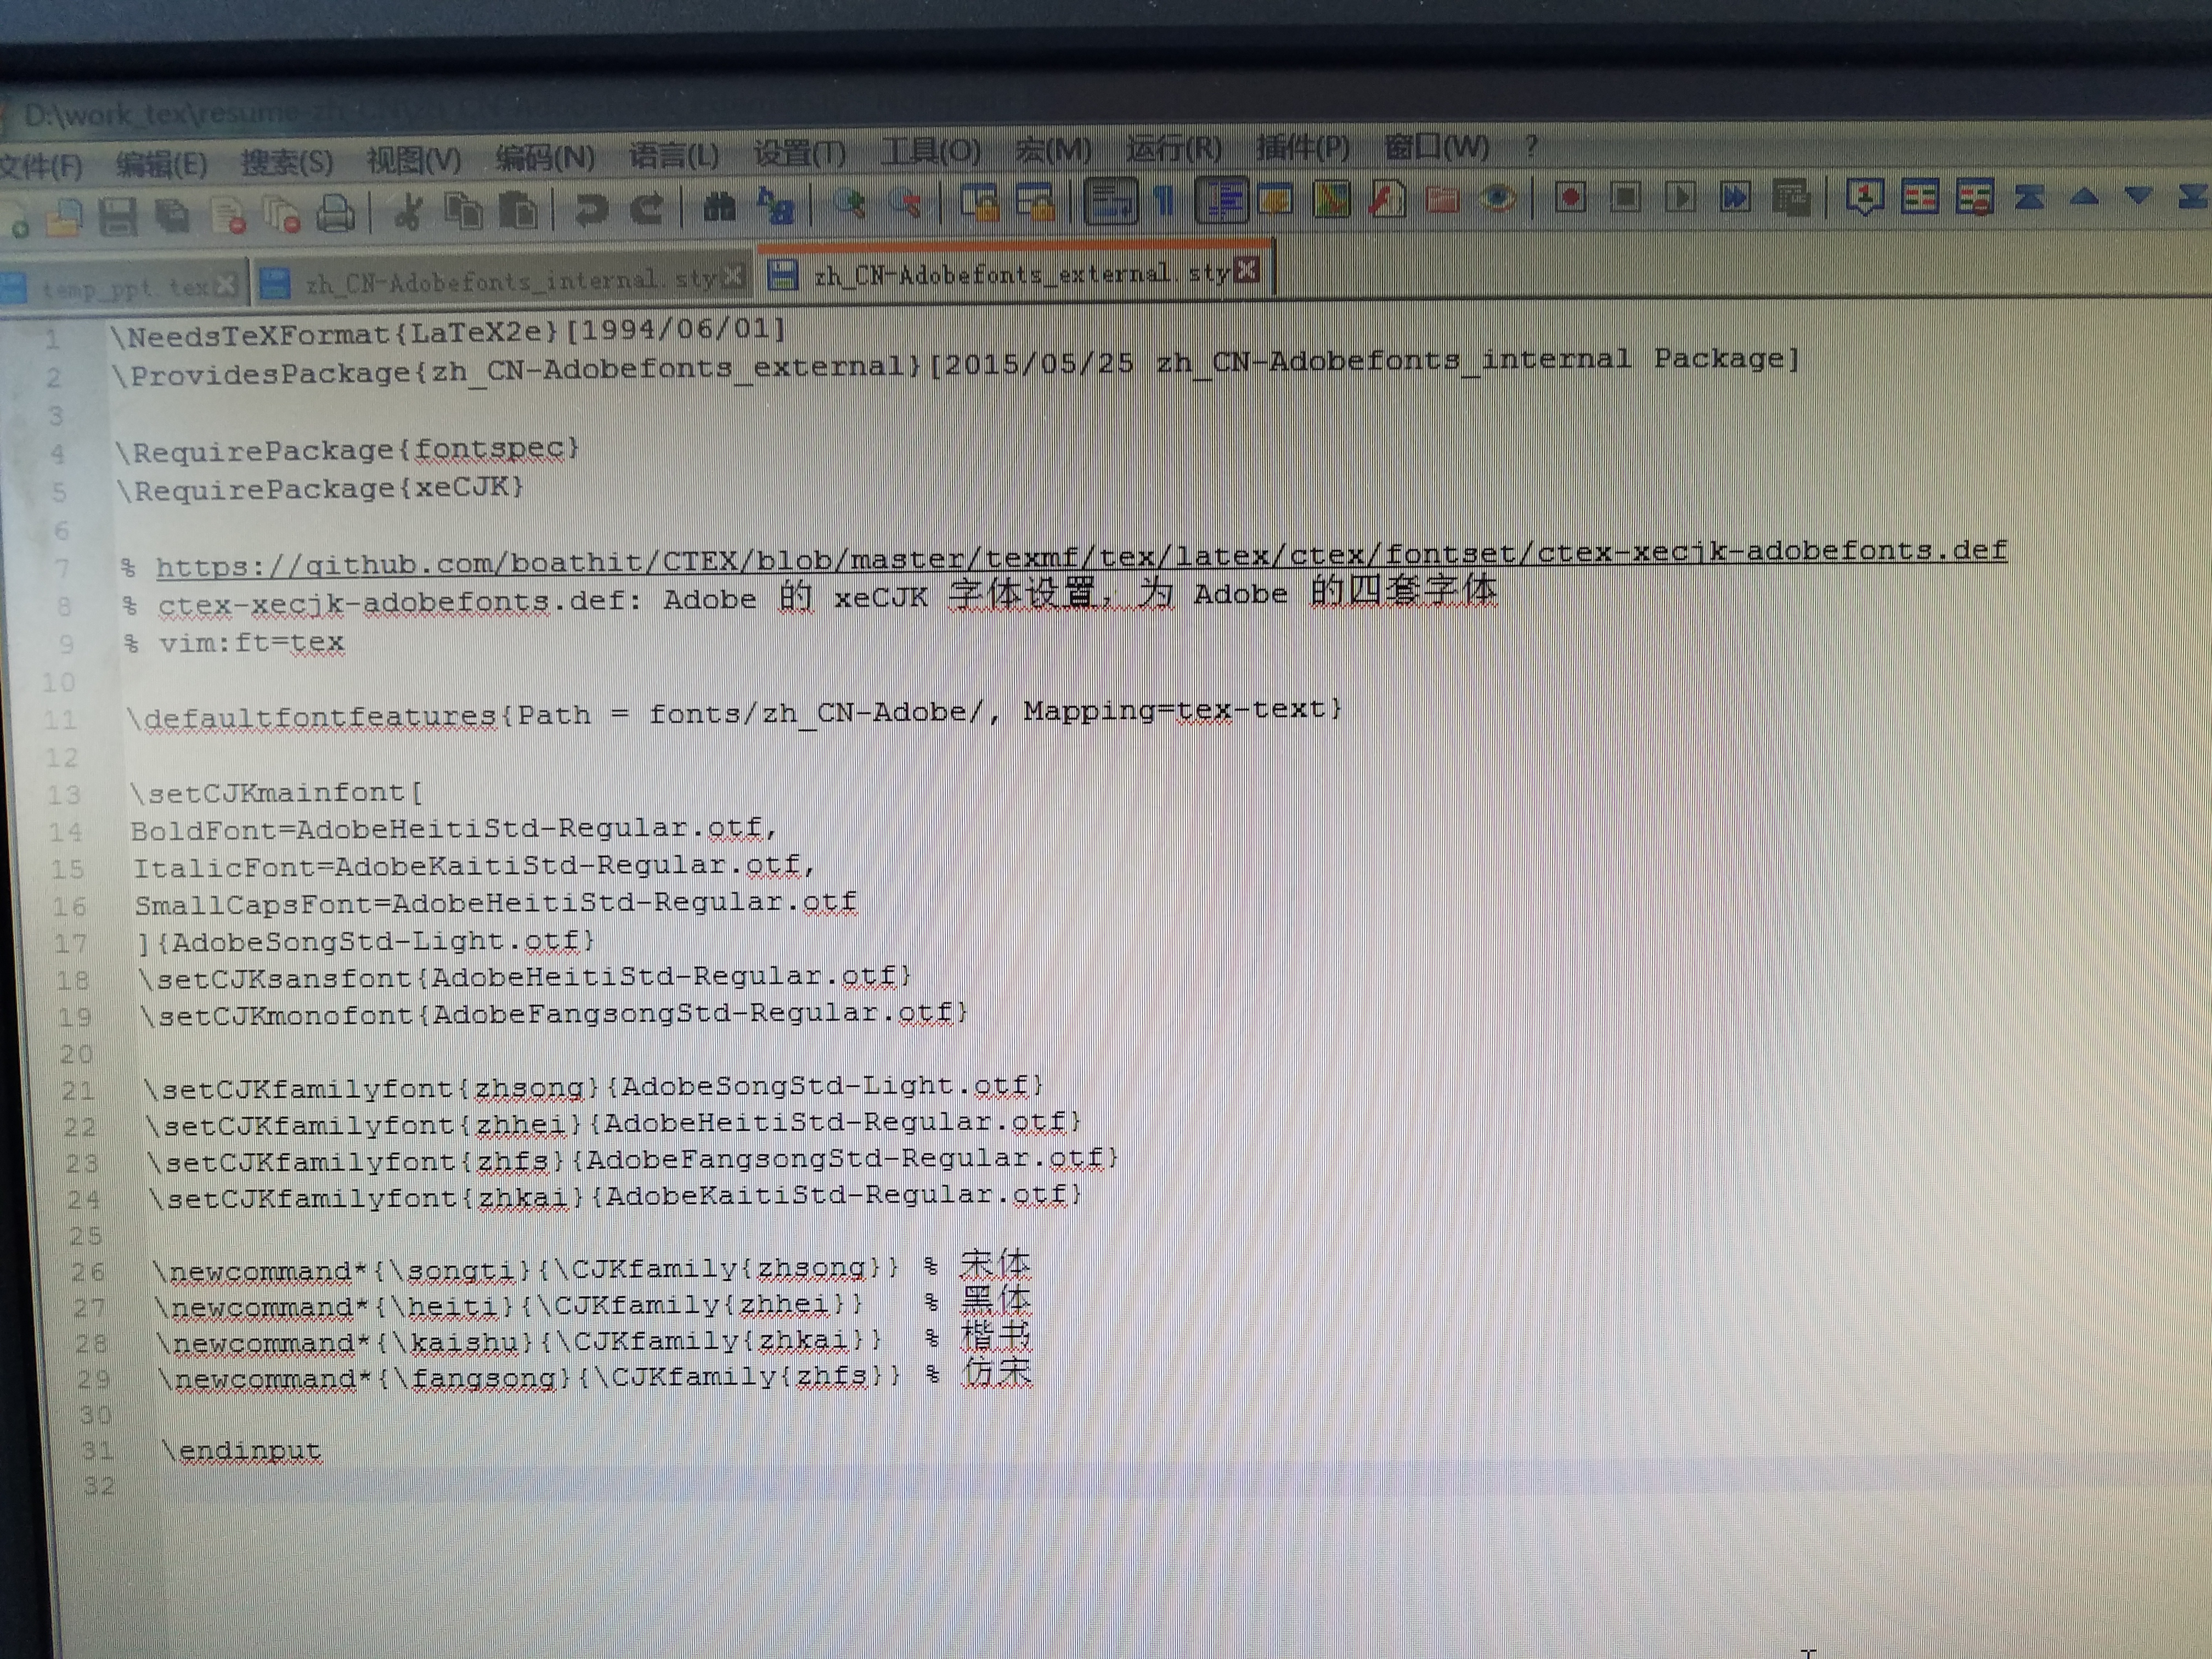
\includegraphics[width=0.65\textwidth]{pic15.jpg}

\begin{qst}\label{Q2018010904}
全角输入法有居中的点吗??\index{间隔号}
\end{qst}
\ans 谷歌输入法,中文输入反单引号(1键左边)就是。

也可以使用\verb|\textperiodcentered |或\verb|\textbullet| 获得文本模式的不同大小的间隔号。
例如:
张三 \textperiodcentered 李四, \quad
王五 \textbullet 赵六

\end{document} 